\documentclass[a4paper, 14pt]{extarticle}
\input{../../.preambles/10-russian}
\input{../../.preambles/20-math}
\usepackage[utf8]{inputenc}
\usepackage[paper=a4paper, top=1cm, right=1cm, bottom=1.5cm, left=2cm]{geometry}
\usepackage{setspace}
\usepackage{ifthen}
\usepackage{array}
\usepackage{bm}
\onehalfspacing

\usepackage{graphicx}
\graphicspath{{plots/}, {images/}}

\parindent=1.25cm

\renewcommand{\thesection}{\arabic{section}.}
\renewcommand{\thesubsection}{\arabic{section}.\arabic{subsection}.}
\numberwithin{equation}{section}

\usepackage{caption}
\DeclareCaptionLabelFormat{figure}{Рисунок #2}
\DeclareCaptionLabelFormat{table}{Таблица #2}
\DeclareCaptionLabelSeparator{sep}{~---~}
\captionsetup{labelsep=sep,justification=centering,font=small}
\captionsetup[figure]{labelformat=figure}
\captionsetup[table]{labelformat=table}

\usepackage{titlesec}
\titleformat{\section}
    {\centering\normalsize\bfseries}
    {\thesection}
    {1em}{}
\titleformat{\subsection}
    {\normalsize\bfseries}
    {\thesubsection}
    {1em}{}

% Настройка вертикальных и горизонтальных отступов
\titlespacing*{\section}{\parindent}{*4}{*4}
\titlespacing*{\subsection}{\parindent}{*4}{*4}

\usepackage[square, numbers, sort&compress]{natbib}
\makeatletter
\bibliographystyle{unsrt}
\renewcommand{\@biblabel}[1]{#1.} 
\makeatother
\addto\captionsrussian{\def\bibname{Список использованных источников}}
\addto\captionsrussian{\def\refname{Список использованных источников}}

\newcolumntype{C}[1]{>{\centering\arraybackslash}m{#1\textwidth}}
\renewcommand{\arraystretch}{1.2}

\usepackage{color}
\definecolor{darkgreen}{rgb}{0,.5,0}
\usepackage[colorlinks,linkcolor=black,filecolor=blue,citecolor=darkgreen,urlcolor=black]{hyperref}

\newcommand{\maketitlepage}[1]{
    \begin{titlepage}
        \singlespacing
        \newpage
        \begin{center}
            Министерство образования и науки Российской Федерации \\
            Федеральное государственное бюджетное образовательное \\
            учреждение высшего профессионального образования \\
            <<Волгоградский государственный технический университет>> \\
            Факультет электроники и вычислительной техники \\
            Кафедра физики
        \end{center}
        \vspace{9em}
        \begin{center}
           { \large\bfseries ОТЧЕТ }
            \\ О научно-исследовательской практике на \( \underset{\text{наименование организации}}{\rule{.35\textwidth}{.5pt}\hrulefill} \)
        \end{center}
        \vspace{4em}
        \begin{table}[h!]
            \center         
            \begin{tabular}{b{.3\textwidth}ccl}
                Руководитель практики от организации & \( \underset{\text{должность}}{\rule{3cm}{.5pt}\hrulefill} \) & \( \underset{\text{подпись}}{\rule{3cm}{.5pt}\hrulefill} \) & Виснер~С.~В. \\
                Руководитель практики от университета & доцент & \( \underset{\text{подпись}}{\rule{3cm}{.5pt}\hrulefill} \) & Поляков~И.~В. \\
                Студент группы Ф-369 & \multicolumn{2}{c}{\( \underset{\text{подпись}}{\rule{6.5cm}{.5pt}\hrulefill} \)} & #1
            \end{tabular}
        \end{table}
        \vspace{5em}

        \begin{flushright}
            \begin{minipage}{.5\textwidth}
                Отчет защищен с оценкой \hrulefill
            \end{minipage}
        \end{flushright}
        \vspace{\fill}
        \begin{center}
            Волгоград, \the\year
        \end{center}

    \end{titlepage}
    \setcounter{page}{2}
}


\begin{document}
\maketitlepage{Слоква~В.~И.}
\setcounter{page}{3}

\section*{Аннотация}

	В данной работе приведены цели и задачи научно-исследовательской практики, а так же приведена топология наиболее распространенных импульсных источников питания. Приведено краткое описание прохождения практики (описаны программы по расчету моточных компонентов, используемые формулы, описание практической части).

\section*{Список ключевых понятий}

Обратноходовый преобразователь, випер, дроссель, трансформатор, мостовой преобразователь, диодный мост, индуктивность.

\newpage

\tableofcontents
\newpage

\phantomsection\addcontentsline{toc}{section}{Введение}
\section*{Введение}

	Прохождение практики студентами на предприятии подразумевает собой ознакомление студентов с реальным технологическим процессом и закреплением теоретических знаний, полученных в ходе обучения.
	
	На протяжении долгого времени остается актуальным вопрос о производстве различных источников питания, ведь от них зависит нормальное функционирование бытовых электроприборов. Каждый год рынок предлагает большое разнообразие подобной продукции, имеющую различные входные и выходные характеристики соответствующие спросу потребителей. К ним относятся источники питания для мобильных устройств, силовая электроника, различные инверторы напряжения и т.п.
	
	В даной работе представлена наиболее распространенная топология импульсных источников питания. А также более детально описан преобразователь с передачей энергии на обратном ходу, т.к. приведенная схема является одной из наиболее часто применяемых в электронике рассматриваемого типа.
\newpage

\section{Основные схематические решения для импульсных источников питания}

\subsection{Понижающий преобразователь мощностью до нескольких киловатт.}

	Понижающий преобразователь (рис.~\ref{p1}) относится к разряду прямоходовых схем. Он позволяет получать выходную мощность в несколько киловатт. Предназначен для использования в тех слу-чаях, когда не нужна изоляция между первичной и вторичной сторонами.
	
	Для повышения эффективности вместо диода может также использоваться транзистор с дополнительной схемой управления, связанной с ШИМ-контроллером (синхронный выпрямитель). 
Применение синхронного выпрямителя позволяет существенно повысить КПД преобразователя. Так, например, в типовом случае понижающий преобразователь без синхронного выпрямителя имеет КПД, 
равный 86\%, а с ним — 95\%. В устройствах, рассчитанных на большие токи потребления (например, в схемах питания процессоров), часто используется 
многофазное преобразование, что позволяет снизить токи пульсаций и тем самым снизить нагрузку на выходные ёмкости и уменьшить габариты индуктора (суммарный объём, занимаемый им на монтаж-ной плате).

\begin{figure}[ht]
	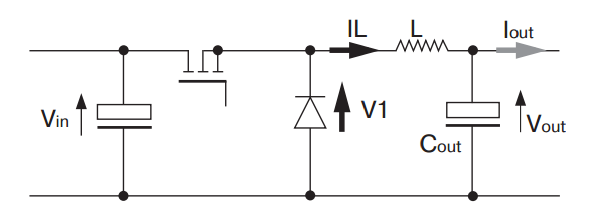
\includegraphics[width=.45\textwidth]{s_01} \hfill
	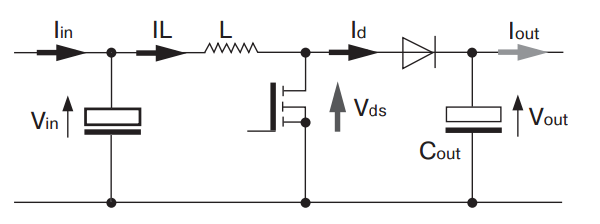
\includegraphics[width=.45\textwidth]{s_02}
	\parbox{.45\textwidth}{\caption{}\label{p1}} \hfill
	\parbox{.45\textwidth}{\caption{}\label{p2}}
\end{figure}

\subsection{Повышающий преобразователь мощностью до нескольких 
киловатт.}

	Повышающий преобразователь (рис.~\ref{p2}) относится к типу обратноходовых схем. Его особенность -- выходное напряжение всегда больше входного.  Выходная мощность может составлять 
сотни ватт в прерывистом режиме и до нескольких 
киловатт в непрерывном режиме.

\subsection{Инвертирующий преобразователь.}

	Инвертирующий преобразователь (рис.~\ref{p3}) также относится к обратноходовым схемам. Его особенность: выходное напряжение преобразователя имеет отрицательную полярность относительно земли.
	 
	Когда ключ замкнут, ток через индуктор линейно растёт и в нем запасается энергия. В момент размыкания ключа напряжение на индукторе меняет знак, ток продолжает течь через диод, заряжая конденсатор. 
Как и рассмотренные выше преобразователи, инвертирующая схема также может работать в режиме непрерывного тока в индукторе и в прерывистом режиме.

\begin{figure}[ht]
	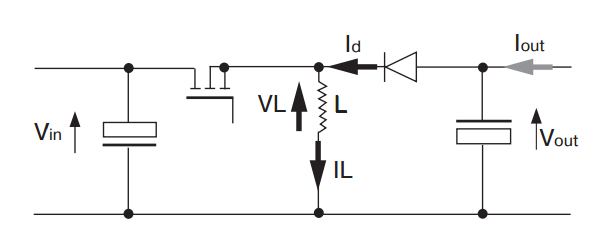
\includegraphics[width=.45\textwidth]{s_03} \hfill
	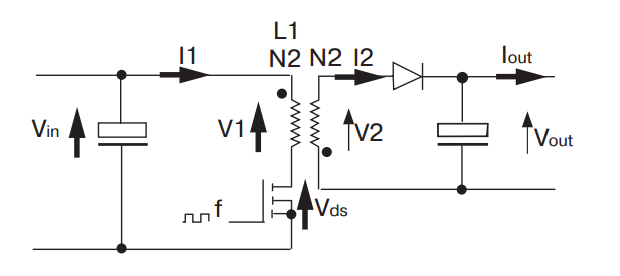
\includegraphics[width=.45\textwidth]{s_04}
	\parbox{.45\textwidth}{\caption{}\label{p3}} \hfill
	\parbox{.45\textwidth}{\caption{}\label{p4}}
\end{figure}

\subsection{Обратноходовой преобразователь мощностью до 200 Вт.}

	Обратноходовой преобразователь (рис.~\ref{p4}) по принципу работы аналогичен повышающему преобразователю (когда ключ находится в открытом состоянии (замкнут), энергия запасается в трансформаторе/индукторе, при разомкнутом ключе энергия передаётся в нагрузку).
	
	Обратноходовой преобразователь может работать как в режиме непрерывного тока в трансформаторе (индукторе), так и в прерывистом режиме. Следует отметить, что в непрерывном режиме схема очень нестабильна и склонна к автогенерации, поэтому преобразователи этого типа в основном проектируют для работы в прерывистом режиме.

\subsection{Прямоходовой преобразователь.}

	В отличие от обратноходовой схемы, в трансформаторе прямоходового преобразователя энергия не запасается (рис.~\ref{p5}). Когда ключ открыт, к первичной обмотке прикладывается напряжение питания $ V_{in} $. На обмотке N2 появляется напряжение, открывается диод D2, ток протекает через индуктор LС-фильтр в нагрузку. Когда ключ размыкается, 
открывается диод D3, энергия, запасённая в индукторе L, поступает в нагрузку. Размагничивание трансформатора происходит через дополнительную обмотку и диод D1.

	Схема может работать как в режиме непрерывно-го тока в индукторе L, так и в прерывистом режиме.

\begin{figure}[ht]
	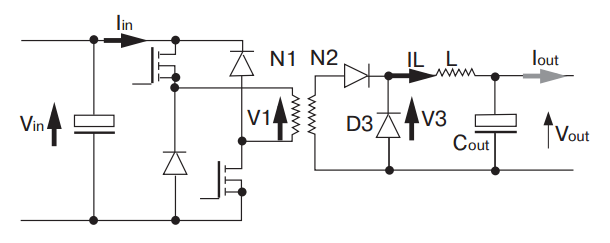
\includegraphics[width=.45\textwidth]{s_05} \hfill
	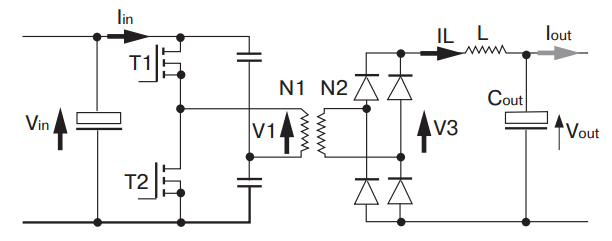
\includegraphics[width=.45\textwidth]{s_06}
	\parbox{.45\textwidth}{\caption{}\label{p5}} \hfill
	\parbox{.45\textwidth}{\caption{}\label{p6}}
\end{figure}

\subsection{Полумостовой преобразователь.}

	Энергия передаётся в нагрузку в течение двух полупериодов цикла. Схема позволяет получать большие выходные мощности (рис.~\ref{p6}). Когда замкнут верхний ключ T1, на первичную обмотку N1 подаётся положительное напряжение, равное $ V_{in}/2 $ (напряжение на конденсаторах делится ровно пополам). На вторичной обмотке появляется положительное напряжение, кратное коэффициенту трансформации, напряжение через диагональ диодного моста поступает на LC- фильтр в нагрузку. Далее выдерживается пауза (<<мёртвое время>>) до полного закрытия верхнего транзистора и открывается нижний транзистор. На первичную обмотку поступает отрицательное напряжение, на вторичной обмотке появляется напряжение также отрицательной полярности и через вторую диагональ поступает через LC-фильтр в нагрузку. 

	Когда ни один из ключей не замкнут (<<мёртвое время>>), индуктор отдаёт в нагрузку накопленную энергию. Если ток в индукторе не падает до нуля, то такой режим работы называется непрерывным, если ток падает до нуля, то это прерывистый режим. Прерывистый режим характеризуется большими токами, что приводит к повышенным потерям мощности в ключах и выходных диодах.
	
\subsection{Мостовой преобразователь.}

	В отличие от полумостовой схемы здесь используются четыре 
транзистора (рис.~\ref{p7}). Мостовой преобразователь применяется в мощных схемах от единиц до десятков киловатт, что позволяет снизить токи в первичной цепи в два раза по сравнению с полумостовой схемой.

	Когда замкнута пара ключей T1 и T4, к первичной обмотке N1 прикладывается напряжение питания $ V_{in} $. На вторичной обмотке N2 появляется напряжение, которое через LC фильтр поступает 
на нагрузку. Затем пара ключей T1 и T4 размыкается, после паузы замыкаются ключи T2 и T3, на первичную обмотку подаётся напряжение питания $ V_{in} $ отрицательной полярности. 

	Как и полумостовая, мостовая схема может работать в непрерывном режиме или в прерывистом.

\begin{figure}[ht]
	\center
	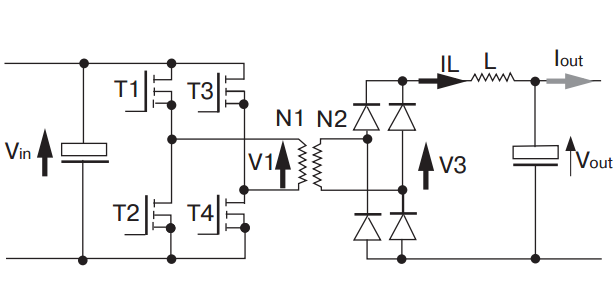
\includegraphics[width=.6\textwidth]{s_07}
	\caption{}\label{p7}
\end{figure}

\section{Практическая часть}
На рис.~\ref{p8} приведена электрическая схема обратноходового преобразователя, базируемого на микросхеме \emph{Viper53}. Данная схема очень удобна для рассмотрения общих схемотехнических принципов, которые легко могут быть применены и в большинстве других случаев.

\begin{table}[h!]
	\center
	\caption{Входные и выходные характеристики} \label{t01}
	\begin{tabular}{|*{6}{C{.15}|}} \hline
		Входное напряжение & Выходное напряжение & Выходной ток & Выходная мощность &
		Частота преобразования & КПД \\ \hline
		220~VAC \( \pm 20\% \) & 12~VDC & 0,6~А & 7,2~Вт & 100~кГц & 80~\% \\ \hline
	\end{tabular}
\end{table}

С учетом входных и выходных данных, а также с помощью использования следующих программ: \emph{Viper Flyback} и \emph{Lite-CalcIT} (2000), была разработана и рассчитана схема импульсного блока питания на 12~В.

\begin{figure}[ht]
	\center
	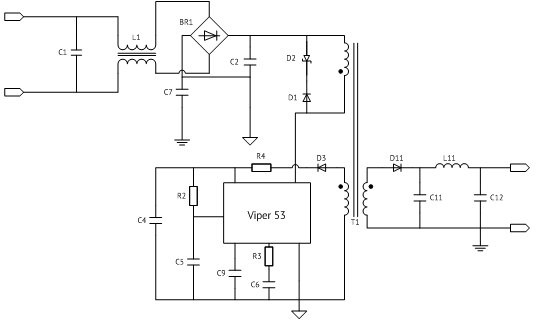
\includegraphics{m_05}
	\caption{Электрическая схема}\label{p05}
\end{figure}

Для проектирования моточных компонентов (трансформаторов, дросселей) были использованы следующие программы: \emph{TransK1.0}, \emph{Forward}, \emph{Flyback}.

Номиналы и наименования компонентов электрической схемы приведены в таблице~\ref{t02}.
\begin{table}[h!]
	\center
	\caption{Номиналы и наименования элементов электрической схемы} \label{t02}
	\begin{tabular}{|*{14}{C{.05}|}} \hline
		\multicolumn{2}{|C{.1}|}{C1} & C2 & C4 & C5 & C6 & \multicolumn{2}{C{.1}|}{C7}
		& C9 & C11 & C12 & R2 & R3 & R4 \\ \hline
		\multicolumn{2}{|C{.1}|}{22 мкФ -- 1~кВ} & 10 мкФ & 4,7 мкФ & 2,2 нФ & 47 нФ
		& \multicolumn{2}{C{.1}|}{2,2 нФ -- 2~кВ} & 22 нФ & 0,33 мФ & 56 мкФ & 6,8 кОм
		& 820 Ом & 10 Ом \\ \hline
	\end{tabular}
	\begin{tabular}{|*{3}{C{.079}|}*{3}{C{.1}|}C{.15}|C{.11}|} \hline
		L1 & L11 & T1 & D1 & D2 & D3 & D11 & BR1 \\ \hline
		6,8 мкГн & 10 мкГн & 1,35 мГн & BYT11 & BZW04-188 & BAS21 & STPS1H100 &
		KC407A \\ \hline
	\end{tabular}
\end{table} 

Рассчитанная схема полностью удовлетворяет заявленным требованиям.

\newpage

\phantomsection\addcontentsline{toc}{section}{Список литературы}
\begin{thebibliography}{9}
	\bibitem{1} Макашов,~Д. Обратноходовый преобразователь [Электронный ресурс]~/
	Д.~Макашов~-- 2005-2006.~-- Режим доступа:
	\href{http://www.bludger.narod.ru/smps/Flyback-R01.pdf}
	{http://www.bludger.narod.ru/smps/Flyback-R01.pdf}
	\bibitem{2} Фролов,~В.~В. Язык радиосхем [Текст]~/ В.~В.~Фролов~-- 2-е изд., перераб.
	и доп.~-- М.: Радио и связь, 1988.~-- 128~c.
	\bibitem{3} Браун,~М. Источники питания. Расчет и конструирование [Текст]~/
	М.~Браун; пер. с англ. С.~Л.~Попова~-- К.: <<МК-Пресс>>, 2007.~-- 288~с.
	\bibitem{4} Мэк,~Р. Импульсные источники питания. Теоретические основы и руководство по практическому применению [Текст]~/
	Р.~Мэк; пер. с англ. С.~В.~Пряничникова~-- М.: Издательский дом <<Додэка-XXI>>, 2008.~-- 272~с.
\end{thebibliography}
\end{document}
